\documentclass{article}

\usepackage{../preamble/factory, ../preamble/font, ../preamble/math, ../preamble/math_font, ../preamble/style, ../preamble/theorem}

\newtheorem{thr}{Uppgift}

\begin{document}

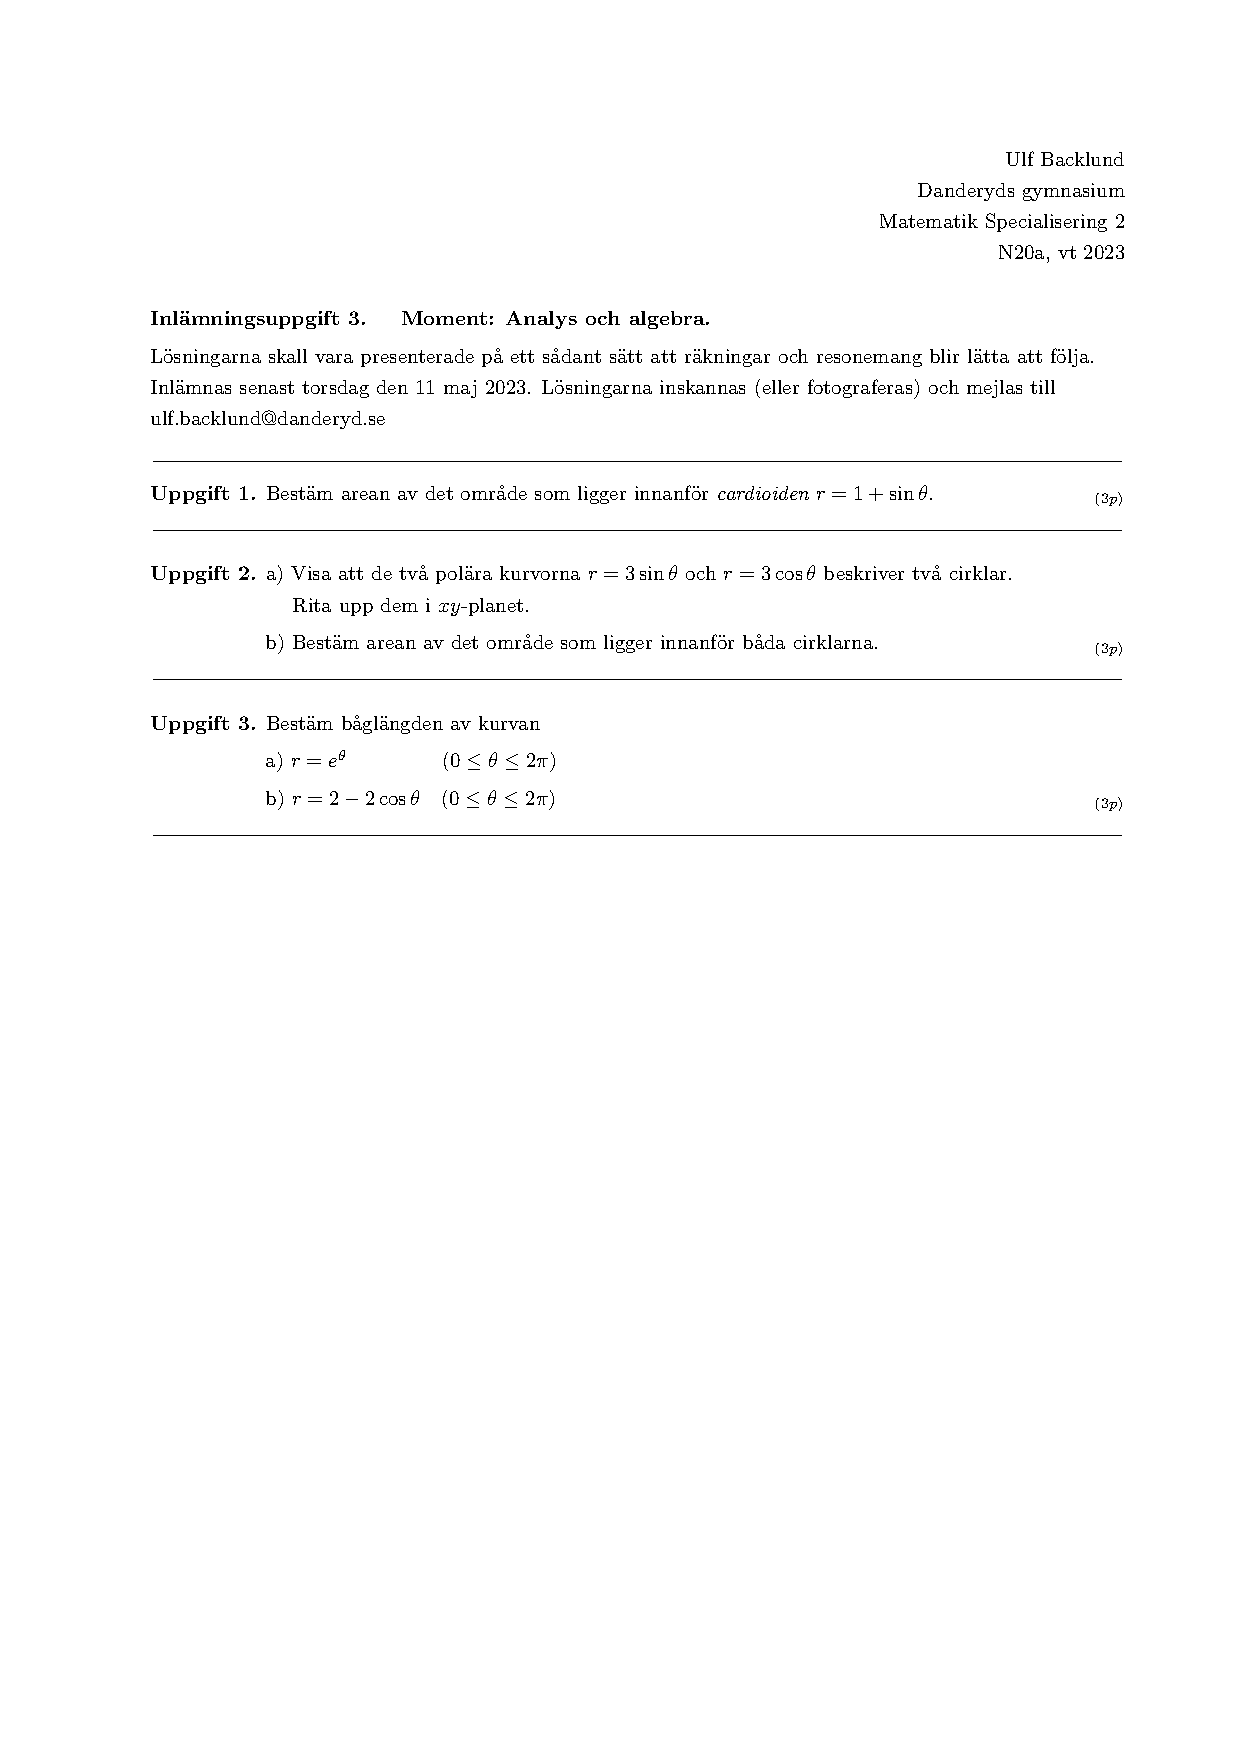
\includepdf{homework_3}

\newpage

\centerline{\large Matematik specialisering 2 inlämning 3}

\vskip 0.1cm

\centerline{\scriptsize Adam Amanbaev}

\begin{thr}
Bestäm arean av det område som ligger innanför cardioiden $r=1+\sin\theta$
\end{thr}

Låt $f(\theta)=r=1+\sin\theta$. Då kan arean, $A$, av det område som ligger innanför cardioiden $f(\theta)$ skrivas som följande:

$$
A=
\int_{\alpha}^{\beta} \frac{f(\theta)^2}{2} \: d\theta
$$

\vskip 0.2cm

Nedan följer en skissering av $f$:

\begin{figure}[h]
    \center
    \begin{tikzpicture}
        \begin{axis}[
            xmin=-2, xmax=2,
            ymin=-1, ymax=2.5,
            axis lines=middle,
            minor tick num=9,
            axis line style={latex-latex},
            ticklabel style={font=\tiny},
            axis equal
            ]

            \addplot[domain=0:360,samples=300,color=red,data cs=polar] (x,{1+sin(x)});

        \end{axis}
    \end{tikzpicture}
\end{figure}

Observerar man figuren för $f$ ovan ser man att $\alpha=0$ och $\beta=2\pi$ ska gälla för att exakt hela området innanför cadioiden ska svepas med formeln för arean. Vi får då följande area:

$$
\therefore 
\;
A=
\int_{0}^{2\pi} \frac{f(\theta)^2}{2} \: d\theta
=
\int_{0}^{2\pi} \frac{(1+\sin\theta)^2}{2} \: d\theta
=
\int_{0}^{2\pi} \frac{1+\sin^2 \theta+2\sin\theta}{2} \: d\theta
$$

$$
=
\frac{1}{2}
\int_{0}^{2\pi} 1+\sin^2 \theta+2\sin\theta \: d\theta
=
\frac{1}{2}
\int_{0}^{2\pi} 1+\frac{1-\cos 2\theta}{2}+2\sin\theta \: d\theta
$$

$$
=
\frac{1}{8}
\int_{0}^{2\pi} 6-2\cos 2\theta+8\sin\theta \: d\theta
=
\frac{1}{8}
\left[6\theta-\sin2\theta-8\cos\theta \right]_{0}^{2\pi}
$$

$$
=
\frac{1}{8}
((12\pi-0-8)-(0-0-8))
= 
\frac{3\pi}{2} \: \text{a.e}
$$

\newpage

\begin{thr}
\end{thr}

\begin{enumerate}
    \item[a)] Vi kan skriva om uttrycken genom att multiplicera dem med $r$:
        $$
        r_1=3\sin\theta 
        \Ekv
        r_{1}^2=3r_{1}\sin\theta
        \Ekv_{\text{def. av polära koordinater}}
        \:
        x^2+y^2=3y
        $$
        $$
        \Ekv
        x^2+(y-\frac{3}{2})^2=(\frac{3}{2})^2
        $$

        $$
        r_2=3\cos\theta 
        \Ekv
        r_{2}^2=3r_{2}\cos\theta
        \Ekv_{\text{def. av polära koordinater}}
        \:
        x^2+y^2=3x
        $$
        $$
        \Ekv
        (x-\frac{3}{2})^2+y^2=(\frac{3}{2})^2
        $$

        \vskip 0.3cm

        Alltså är polära kurvan $r_{1}=3\sin\theta$ ekvivalent med cirkeln $x^2+(y-\frac{3}{2})^2=(\frac{3}{2})^2$ och polära kurvan $r_{2}=3\cos\theta$ är ekvivalent med cirkeln $(x-\frac{3}{2})^2+y^2=(\frac{3}{2})^2$. $r_{1}$ och $r_{2}$ skisseras i följande figure i blått respektive rött:

        \begin{figure}[h]
            \center
            \begin{tikzpicture}
                \begin{axis}[
                    xmin=-4, xmax=4,
                    ymin=-4, ymax=4,
                    axis lines=middle,
                    minor tick num=9,
                    axis line style={latex-latex},
                    ticklabel style={font=\tiny},
                    axis equal
                    ]

                    \addplot[domain=0:360,samples=300,color=blue,data cs=polar] (x,{3*sin(x)});
                    \addplot[domain=0:360,samples=300,color=red,data cs=polar] (x,{3*cos(x)});

                \end{axis}
            \end{tikzpicture}
        \end{figure}

    \item[b)] Vi observerar först vinkeln i första kvadranten där de två polära kurvorna korsar varandra:
        $$
        r_{1}=r_{2}
        \Ekv
        3\sin\theta=3\cos\theta
        \Ekv
        \sin\theta=\cos\theta
        \Imp_{\text{kvadr. I}}
        \;
        \theta=\frac{\pi}{4}
        $$

        För att beräkna arean av området som täcks av båda cirklarna beräknar vi ut arean av området som sveps av $r_{2}$ då $\frac{\pi}{4}\leq\theta\leq\frac{\pi}{2}$ samt arean av området som sveps av $r_{1}$ då $0\leq\theta\leq\frac{\pi}{4}$. Dessa skisseras i följande figur i rött respektive blått:

        \newpage

        \begin{figure}[h]
            \center
            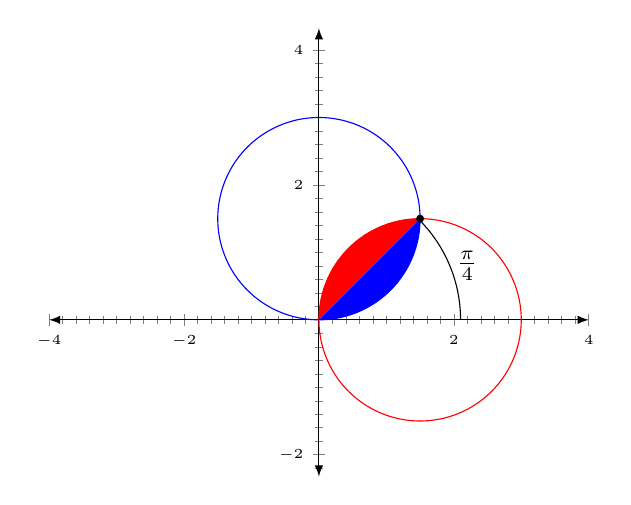
\begin{tikzpicture}
                \begin{axis}[
                    xmin=-4, xmax=4,
                    ymin=-2, ymax=4,
                    axis lines=middle,
                    minor tick num=9,
                    axis line style={latex-latex},
                    ticklabel style={font=\tiny},
                    axis equal
                    ]

                    \addplot[domain=0:360,samples=300,color=blue,data cs=polar] (x,{3*sin(x)});
                    \addplot[domain=0:360,samples=300,color=red,data cs=polar] (x,{3*cos(x)});
                    \fill[fill=red] plot[domain=pi/4:pi/2] (xy polar cs:angle=\x r, radius={3*cos(\x r)});
                    \fill[fill=blue] plot[domain=0:pi/4] (xy polar cs:angle=\x r, radius={3*sin(\x r)});
                    \draw[black, fill=black] (1.5, 1.5) circle(0.05);
                    \draw (2.1, 0) arc (0: 45: 2.1);
                    \draw (2.2, 0.8) node {$\frac{\pi}{4}$};
                \end{axis}
            \end{tikzpicture}
        \end{figure}

        Låt arean av det röda området vara $A_{r_{2}}$ och arean av det blåa området vara $A_{r_{1}}$. Då gäller följande:

        $$
        A_{r_{2}}
        =
        \int_{\frac{\pi}{4}}^{\frac{\pi}{2}} \frac{(r_{2})^2}{2} \; d\theta
        =
        \int_{\frac{\pi}{4}}^{\frac{\pi}{2}} \frac{(3\cos\theta)^2}{2} \; d\theta
        =
        \frac{9}{8}
        \int_{\frac{\pi}{4}}^{\frac{\pi}{2}} 4\cos^2\theta \; d\theta
        $$
        $$
        =
        \frac{9}{8}
        \int_{\frac{\pi}{4}}^{\frac{\pi}{2}} 2+2\cos2\theta \; d\theta
        =
        \frac{9}{8}
        \left[2\theta+\sin2\theta \; \right]_{\frac{\pi}{4}}^{\frac{\pi}{2}}
        $$
        $$
        =
        \frac{9}{8}
        ((\pi+0)-(\frac{\pi}{2}+1))
        =
        \frac{9\pi-18}{16} \: \text{a.e}
        $$

        $$
        A_{r_{1}}
        =
        \int_{0}^{\frac{\pi}{4}} \frac{(r_{1})^2}{2} \; d\theta
        =
        \int_{0}^{\frac{\pi}{4}} \frac{(3\sin\theta)^2}{2} \; d\theta
        =
        \frac{9}{8}
        \int_{0}^{\frac{\pi}{4}} 4\sin^2\theta \; d\theta
        $$
        $$
        =
        \frac{9}{8}
        \int_{0}^{\frac{\pi}{4}} 2-2\cos2\theta \; d\theta
        =
        \frac{9}{8}
        \left[2\theta-\sin2\theta \; \right]_{0}^{\frac{\pi}{4}}
        $$
        $$
        =
        \frac{9}{8}
        ((\frac{\pi}{2}-1)-(0-0))
        =
        \frac{9\pi-18}{16} \: \text{a.e}
        $$

        Arean av området som täcks av båda cirklarna $r_{1}$ och $r_{2}$ blir då $A=A_{r_{1}}+A_{r_{2}}$.

        $$
        \therefore
        \;
        A
        =
        A_{r_{1}}+A_{r_{2}}
        =
        \frac{9\pi-18}{16}+\frac{9\pi-18}{16}
        =
        \frac{9\pi-18}{8} \: \text{a.e}
        $$

\end{enumerate}

\newpage

\begin{thr}
\end{thr}

Båglängden $s$ av en polär kurva, $\alpha\leq\theta\leq\beta$, kan bestämmas med följande uttryck:

$$
s
=
\int_{\alpha}^{\beta} \sqrt{(\frac{dr}{d\theta})^2+r^2} \: d\theta
$$

\vskip 0.5cm

\begin{enumerate}
    \item[a)] 
        $$
        \therefore
        \;
        s
        =
        \int_{0}^{2\pi} \sqrt{(\frac{d(e^{\theta})}{d\theta})^2+(e^{\theta})^2} \: d\theta
        =
        \int_{0}^{2\pi} \sqrt{e^{2\theta}+e^{2\theta}} \: d\theta
        =
        \int_{0}^{2\pi} \sqrt{2}e^{\theta} \: d\theta
        $$

        $$
        =
        \sqrt{2}
        \int_{0}^{2\pi} e^{\theta} \: d\theta
        =
        \sqrt{2}
        \left[e^\theta \right]_{0}^{2\pi}
        =
        \sqrt{2}
        (e^{2\pi} - 1)
        =
        \sqrt{2}e^{2\pi}-\sqrt{2} \: \text{l.e}
        $$

        $$
        \therefore
        \;
        \text{Båglängden av $r=e^{\theta}, 0\leq\theta\leq2\pi$ är alltså $\sqrt{2}e^{2\pi}-\sqrt{2} \: \text{l.e}$}
        $$

    \item[b)]
        $$
        \therefore
        \;
        s
        =
        \int_{0}^{2\pi} \sqrt{(\frac{d(2-2\cos\theta)}{d\theta})^2+(2-2\cos\theta)^2} \: d\theta
        $$

        $$
        =
        \int_{0}^{2\pi} \sqrt{4\sin^2\theta+4\cos^2\theta-8\cos\theta+4} \: d\theta
        =
        \int_{0}^{2\pi} \sqrt{8-8\cos\theta} \: d\theta
        \;\;
        \text{(\emph{trig. ettan})}
        $$

        $$
        = 
        4
        \int_{0}^{2\pi} \sqrt{\frac{1-\cos\theta}{2}} \: d\theta
        =
        4
        \int_{0}^{2\pi} \sqrt{\sin^2(\frac{\theta}{2})} \: d\theta
        =
        4
        \int_{0}^{2\pi} \sin(\frac{\theta}{2}) \: d\theta
        $$

        $$
        =
        4
        \left[-2\cos(\frac{\theta}{2}) \right]_{0}^{2\pi}
        =
        4
        (2-(-2))
        =
        16 \: \text{l.e}
        $$

        $$
        \therefore
        \;
        \text{Båglängden av $r=2-2\cos\theta, 0\leq\theta\leq2\pi$ är alltså 16 l.e}
        $$

\end{enumerate}

\end{document}
